\thispagestyle{fancy}
\fancyhf{}
\fancyfoot[L]{\thepage}
\renewcommand{\headrulewidth}{0pt}
\renewcommand{\footrulewidth}{0pt}
\footskip = 0pt

\setcounter{page}{48}
\begin{figure*}[ht!]
\centering
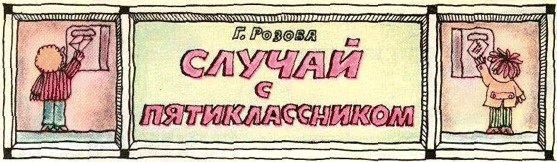
\includegraphics[width=0.95\linewidth]{picture.jpg}
\end{figure*}
\begin{minipage}[bs]{0.44\textwidth}
Все началось с писем.

\quad П и с ь м о\quad п е р в о е.\qquad«Здравствуй, Андрей! У нас в школе недавно была олимпиада по математике. Я решил все задачи, только в последней я не уверен. Некогда было проверить, все ли числа я нашел; да если бы и было время — все равно не стал бы перебирать все двузначные числа, потому что скучно это! Порешай и напиши, какие у тебя будут ответы, а то я сомневаюсь. Вот эта задача.

\qquad\textit{В некотором двузначном числе зачеркнули цифру, и оно уменьшилось в 31 раз. Какую цифру и в каком числе зачеркнули?}

\qquadУ меня получилось три ответа: 31, 62, и 93, причем зачеркивать надо первую цифру. Сергей».


\qquadП и с ь м о\quadв т о р о е.\quad«Здравствуй, Сережа. Ты дал правильный ответ и, если ты так догадлив, то реши нашу олимпиадную задачу.

\qquad\textit{Трехзначное число больше двузначного, записанного его последними цифрами, в 26 раз. Найти это число.
Сколько всего существует таких чисел?} Андрей».

\qquadПолучив это письмо, Сережа обрадовался, а потом попробовал решить задачу Андрея. Но на этот раз догадка не приходила, хотя Сережа испытал много чисел, пробовал составлять их сам. Тогда он подумал, что, может быть, задачу можно решить уравнением. Но что принять за х? Трехзначное число? А как тогда записать условие задачи?

\qquadВдруг его «осенило», что все числа записываются с помощью лишь десяти цифр. В задаче неизвестно трехзначное число. Вот и три неизвестных:

\qquadчисло сотен — х,

\qquadчисло десятков — у,

\qquadчисло единиц — г.
\end{minipage}
\qquad 
\begin{minipage}[bs]{0.48\textwidth}
\begin{minipage}[bs]{\textwidth}
\raggedright{А условие задачи запишется так:\\}
{\centering$100x + 10y + z = 26(10y + z),$\\}
\raggedright{или, после упрощений,\\}
{\centering$4x = 10y + z$.

}
Тут Сережа снова призадумался — уравнение одно, а неизвестных три. Но как только он вспомнил, что \textit{х, у, z} — цифры, дело опять пошло. В последнем равенстве справа стоит $10y + z$ — двузначное число, значит и слева 4\textit{х} — тоже двузначное число. Так будет лишь при \textit{х} = 3, 4, \ldots, 9. И сразу получается ответ:
\end{minipage}\\
\newline \\*
\renewcommand{\arraystretch}{0.8}
\renewcommand{\tabcolsep}{0.5cm}
{\small\begin{tabular*}{\textwidth}{@{\extracolsep{\fill}}c|c|c|c|c}
 \hline
 \rule{0cm}{0.65cm}
 \quad\textit{x} & $10y+z$ & \textit{y} & \textit{z} & Ответ\\ [0.3cm]
 \hline
 \rule{0cm}{0.65cm}
 \quad3 & 12 & 1 & 2 & 312 \\
 \quad4 & 16 & 1 & 6 & 416 \\
 \quad5 & 20 & 2 & 0 & 520 \\
 \quad6 & 24 & 2 & 4 & 624 \\
 \quad7 & 28 & 2 & 8 & 728 \\
 \quad8 & 32 & 3 & 2 & 832 \\
 \quad9 & 36 & 3 & 6 & 936 \\ [0.3cm]
 \hline
\end{tabular*}}\\
\newline \\*
\begin{minipage}[bs]{\textwidth}
\qquad Теперь уже Сережа не сомневался, что нашел все числа. Потом он и свою задачу проверил, а Андрея попросил прислать еще задачи. Вот они.

{\small\qquad Задачи

\qquad 1. Найти все двузначные числа, которые делятся нацело на а) 2; б) 3; в) 4; г) 5; д) 6; е) 7; ж) 8; з) 9. и при этом дают частные, равные сумме цифр делимого.

\qquad 2. В записи трехзначного числа все цифры различны и нуля среди них нет. Цифры этого числа начали менять местами, и все получающиеся при этом (различные) трехзначные числа сложили. Доказать, что эта сумма делится на 222.

\qquad Верно ли это утверждение, если в записи исходного трехзначного числа встречаются одинаковые цифры или есть нуль?

\qquad 3. При делении некоторого двузначного числа на. 6 в остатке получилось число, равное первой цифре делимого, а при делении того же числа на 10 остаток был равен второй цифре числа, а частное — 3. Найти все такие числа.}
\end{minipage}
\end{minipage}

